\documentclass{article}
\usepackage[usenames,dvipsnames]{color} % Required for custom colors
\usepackage{graphicx} % Required to insert images
\usepackage{listings} % Required for insertion of code
\usepackage{amsmath} % Required for some math formulas
\usepackage{enumitem} % Required for customed enum
\usepackage{url} % Auto line break in URL
\def\UrlBreaks{\do\[\do\\\do\]\do\^\do\_\do\`\do\.\do\@\do\\\do\/\do\!\do\_\do\|\do\;\do\>\do\]\do\)\do\,\do\?\do\'\do+\do\=\do\#}

% Uncomment the lines below if you wish to use Chinese characters
\usepackage{fontspec}  % Chinese characters support
\usepackage{indentfirst} % Add indent at the first paragraph
\XeTeXlinebreaklocale "zh" % Automatic line break
\XeTeXlinebreakskip = 0pt plus 1pt % Automatic line break
\setmainfont{Adobe Fangsong Std} % Use a Chinese font
% Use Chinese for figure name
\renewcommand\figurename{图}

%----------------------------------------------------------------------------------------
%	TITLE SECTION
%----------------------------------------------------------------------------------------

\newcommand{\horrule}[1]{\rule{\linewidth}{#1}} % Create horizontal rule command with 1 argument of height

\title{	
\normalfont \normalsize 
% \textsc{university, school or department name} \\ [25pt] % Your university, school and/or department name(s)
\horrule{0.5pt} \\[0.4cm] % Thin top horizontal rule
\huge 光线追踪项目报告 \\ % The assignment title
\horrule{2pt} \\[0.5cm] % Thick bottom horizontal rule
}

\author{胡津铭} % Your name

\date{\normalsize\the\year 年\the\month 月\the\day 日} % Today's date or a custom date

%----------------------------------------------------------------------------------------
%	CODE INCLUSION CONFIGURATION
%----------------------------------------------------------------------------------------

\definecolor{MyDarkGreen}{rgb}{0.0,0.4,0.0} % This is the color used for comments
\lstloadlanguages{C++} % Load C++ syntax for listings, for a list of other languages supported see: ftp://ftp.tex.ac.uk/tex-archive/macros/latex/contrib/listings/listings.pdf
\lstset{language=C++, % Use C++ in this example
        frame=single, % Single frame around code
        basicstyle=\small\ttfamily, % Use small true type font
        keywordstyle=[1]\color{Blue}\bf, % C++ functions bold and blue
        keywordstyle=[2]\color{Purple}, % C++ function arguments purple
        keywordstyle=[3]\color{Blue}\underbar, % Custom functions underlined and blue
        identifierstyle=, % Nothing special about identifiers                                         
        commentstyle=\usefont{T1}{pcr}{m}{sl}\color{MyDarkGreen}\small, % Comments small dark green courier font
        stringstyle=\color{Purple}, % Strings are purple
        showstringspaces=false, % Don't put marks in string spaces
        tabsize=5, % 5 spaces per tab
        %
        % Put standard C++ functions not included in the default language here
        morekeywords={rand},
        %
        % Put C++ function parameters here
        morekeywords=[2]{on, off, interp},
        %
        % Put user defined functions here
        morekeywords=[3]{test},
       	%
        morecomment=[l][\color{Blue}]{...}, % Line continuation (...) like blue comment
        numbers=left, % Line numbers on left
        firstnumber=1, % Line numbers start with line 1
        numberstyle=\tiny\color{Blue}, % Line numbers are blue and small
        stepnumber=5 % Line numbers go in steps of 5
}

% Creates a new command to include a C++ script, the first parameter is the filename of the script (without .pl), the second parameter is the caption
\newcommand{\cppscript}[2]{
\begin{itemize}
\item[]\lstinputlisting[caption=#2,label=#1]{#1}
\end{itemize}
}

\begin{document}
\maketitle % Print the title

\section{简介}
本项目实现了一个较复杂的光线追踪程序。%
能够按照输入的场景描述文件进行计算,生成场景图片,%
并能将多张图片合成为视频。%
主要功能有普通光线追踪、场景运动、物体表面材质、表面纹理、景深效果、%
抗锯齿、八叉树加速、多线程加速、OBJ文件支持等。

\section{算法}
\subsection{光线模型和颜色模型}
每条光线除了记录其起点和方向这两个基本信息外,%
还记录光线的折射率(即目前所处介质中的折射率)和强度。%
这种较复杂的光线模型更接近现实,%
在实现折射和光线混合时更容易处理。%

颜色模型中除了记录RGB值之外,还记录颜色的权重。%
在颜色混合时按照颜色权重的比例加权混合。%
由于物体表面某点的颜色由其漫反射、环境光、镜面反射光线、%
折射光线共同决定,这种模型在混合这些光线时尤为方便。%

\subsection{普通光线追踪}
基本流程如下:
\begin{enumerate}
\item
对于图片的每一个像素点,从视点发出一条光线,光线强度为默认值。
\item
遍历范围内的每一个物体,找到与该光线相交的最近的物体。
\item
根据Phong模型计算交点的颜色值,按光线强度加权。
\item
计算在该点的折射光线及其强度。若不发生全发射则递归跟踪;%
否则将折射强度加给反射强度。
\item
计算在该点的反射光线及其强度,并递归跟踪。
\end{enumerate}

\subsection{纹理}
共提供4种纹理填充方式:Stretch(拉伸)、Tile(平铺)、%
PreserveAspectFit(拉伸时缩放,总是显示完整的图片)、%
PreserveAspectCrop(拉伸时缩放,可能剪裁图片)。%
后两种填充方式在渲染场景中没有用到,故未实现,但预留了接口。%

纹理图片左上角为原点,水平向右为$x$轴,竖直向下为$y$轴。%
填充矩形时,以矩形$v_0$为原点,$\overrightarrow{v_0v_1}$方向为$x$轴,%
$\overrightarrow{v_0v_3}$方向为$y$轴,映射到纹理图片中。%
填充三角形时,以三角形$v_0$为原点,$\overrightarrow{v_1v_0}$方向为$x$轴,%
三角形所在平面内垂直于$x$轴且指向$v_2$一侧为$y$轴,映射到纹理图片中。%
填充球面时,设球心为$O$,球面上一点为$P$,%
$\overrightarrow{OP}$的仰角为$\theta$,方位角为$\phi$,映射方程为:%
$\left\{
\begin{aligned}
x & = \dfrac{\arcsin\left(\dfrac{2\theta}{\pi}-1\right)}{\pi}+\dfrac{1}{2} \\
y & = \dfrac{\arcsin\left(\dfrac{\phi}{\pi}-1\right)}{\pi}+\dfrac{1}{2}
\end{aligned}
\right.
$。
\subsection{八叉树}
建立八叉树的过程如下:
\begin{enumerate}
\item
设定场景的最大范围,并以此为根结点范围建立一个立方体。
\item
不断地向树中加入物体,若某个立方体内的物体数达到临界值,%
则将该立方体均等分为8个小立方体,每个立方体为原立方体的子节点,%
并将原立方体中的物体加入到这些小立方体中。
\end{enumerate}

八叉数的搜索过程如下:
\begin{enumerate}
\item
从根结点开始,进行2。
\item
若当前节点为叶子节点则转3。找到光线最先相交的子节点,转2。
\item
对该节点内的所有物体求交,返回最近相交的物体。
\end{enumerate}

\subsection{多线程加速}
光线追踪算法具有原生的可并行性,采用多线程加速渲染是很好的加速方法。%

\subsection{景深}
实现景深效果需要预先设定照相机的焦距,%
光线追踪时首先求原始光线与焦平面的交点$P_1$和屏幕的交点$P_2$,%
再在$P_2$附近随机选取若干点$P'$,追踪从$P'$到$P_1$的光线,%
最后取平均值作为结果。%
选取的随机点数量越多噪音越小,但计算量越大。

\subsection{抗锯齿}
分别尝试采用最临近插值法、双线性插值法、面积相关重采样法、%
双三次插值法和$Lanczos$插值法5种方法对图像进行模糊以消除锯齿。%

\subsection{OBJ文件支持}
本次作业所提供的OBJ文件样例所涉及到的功能有限,%
所提供的Parser仅支持点和面等简单功能的解析。%
故本程序中重新定义了OBJ Parser,支持纹理、材质等各种功能的解析。%
但本程序中表示材质的参数较多,故本程序中的OBJ Parser不能完全支持标准OBJ文件,%
但能完全支持本次作业中提供的OBJ文件。

\section{运行效果}
\subsection{基本}
普通光线追踪、场景运动、纹理、材质等运行效果见附带示例图片和演示视频。

\subsection{加速}
八叉数加速在物体数目较多时效果非常明显,但在物体数目很少时甚至更慢。%
使用OpenMP并行加速,调度方式采用动态按行分配,%
区块大小为1时加速效果较理想。%
在测试机上运行时加速比约为4.06,效率约为0.51。

\subsection{景深}
采用上述景深算法效果良好,见示例图。

\begin{figure}[!htbp]
    \centering
    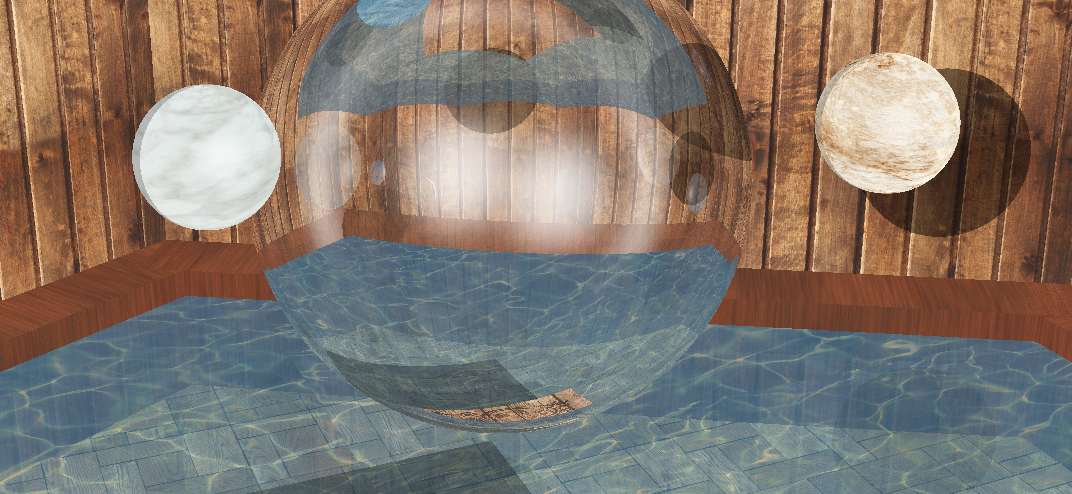
\includegraphics[width=\columnwidth]{org2}
    \caption{未使用景深算法}\label{fig:dofcon}
\end{figure}

图\ref{fig:dofcon}为未使用景深算法时的效果,无论距离远近都能成清晰的像。

\begin{figure}[!htbp]
    \centering
    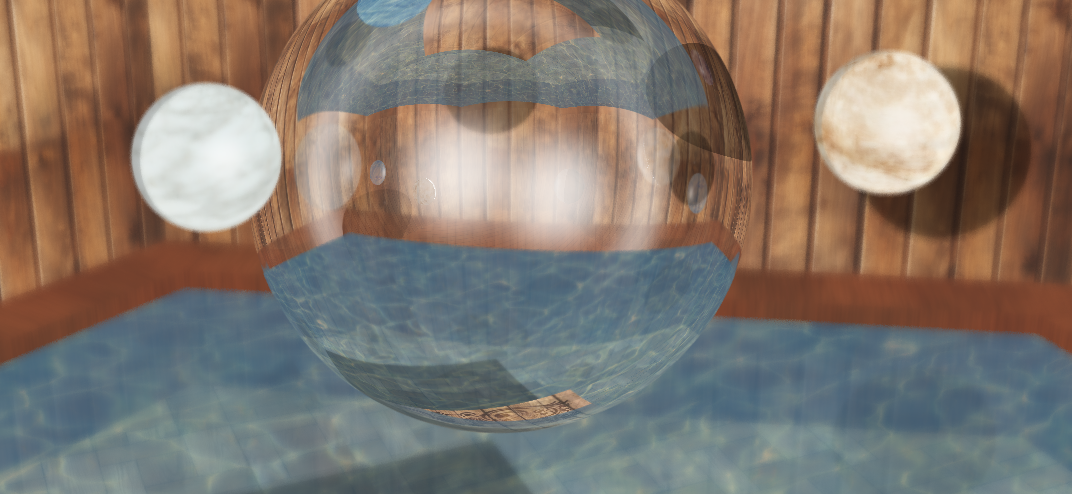
\includegraphics[width=\columnwidth]{dof2}
    \caption{使用景深算法}\label{fig:dof}
\end{figure}

图\ref{fig:dof}是使用景深算法后效果图。%
图中照相机焦点在中心透明球心处,焦点附近成像清晰,%
距离较远或较近处都有不同程度的模糊。

\subsection{抗锯齿}
采用上述抗锯齿算法中的面积相关重采样法效果最好,见示例图片。

\begin{figure}[!htbp]
    \centering
    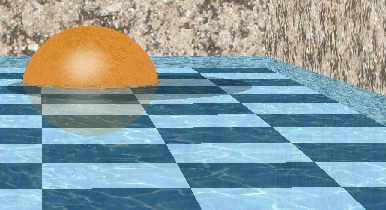
\includegraphics[width=\columnwidth]{org}
    \caption{未使用抗锯齿}\label{fig:aa0con}
\end{figure}

图\ref{fig:aa0con}中,黄色的球边缘及其阴影边缘,地板黑白交界处,均有明显的锯齿。

\begin{figure}[!htbp]
    \centering
    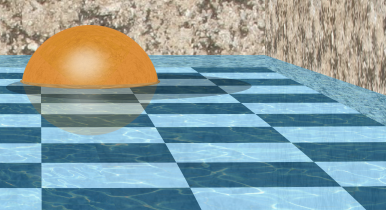
\includegraphics[width=\columnwidth]{aa}
    \caption{使用抗锯齿}\label{fig:aa0}
\end{figure}

图\ref{fig:aa0}中使用抗锯齿算法之后已经找不到锯齿。

\begin{figure}[!htbp]
    \centering
    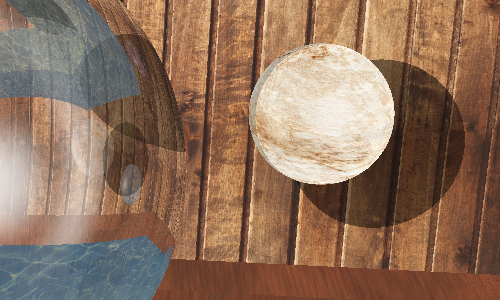
\includegraphics[width=\columnwidth]{org1}
    \caption{未使用抗锯齿}\label{fig:aa1con}
\end{figure}

图\ref{fig:aa1con}中未使用抗锯齿,球边缘以及墙壁直线边缘处有明显的锯齿。

\begin{figure}[!htbp]
    \centering
    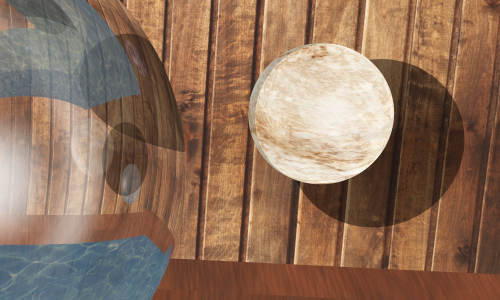
\includegraphics[width=\columnwidth]{aa1}
    \caption{使用抗锯齿}\label{fig:aa1}
\end{figure}

图\ref{fig:aa1}中使用抗锯齿之后已经完全看不到任何锯齿。

注:不同PDF渲染引擎可能会导致不同的显示效果,请参考附带的BMP文件,%
勿以本文档中的图片效果为唯一评价标准。

\section{源文件}
main.cc 主函数

common.h 通用声明和定义

vector3.h 三维向量类,具有加、减、内积、外积计算等功能

color.h 带权RGB颜色类

ray.h 光线类,包括光线起点、方向、光强、所在介质折射率

material.h 材质类,包含多个参数

texture.h 纹理类,包含一个图片和填充方式

object.h 表示物体的抽象基类,包含物体的纹理和材质和一些接口

triangle.h Object基类的派生类,表示一个三角形

rectangle.h Object基类的派生类,表示一个矩形

sphere.h Object基类的派生类,表示一个球体

lightsource.h 点光源类

scene.h 场景类,实现光线追踪的方法

camera.h 照相机类,计算初始光线

octree.h 八叉树

parser.h OBJ文件、CMR文件解析类

\section{编译和运行}
\subsection{编译}
编译需要OpenCV2.0及以上版本链接库,编译器需支持C++11%
(建议GCC 4.8及以上,%
Visual Studio 2012内置MSVC++ 11.0仅部分支持C++11,可能不能通过编译)。%
若要多线程加速,还需要OpenMP链接库。

\subsection{运行}
运行命令为RayTracer OBJFILE CMRFILE OUTPUT。

RayTracer为可执行文件,OBJFILE为场景文件,CMRFILE为照相机参数文件,%
OUTPUT为输出文件。下面是详细的文件语法说明,参数类型默认为浮点型。

\subsubsection{OBJ文件说明}
OBJ文件语法与标准OBJ语法大同小异,扩展了一些功能。%
\begin{enumerate}
\item
以\#为行首的是注释。
\item
以v为行首附带3个数字表示一个顶点。%
\item
以f为行首附带一个数字表示光源,数字(整形)表示光源位置点的编号(从0计,下同);%
附带两个数字表示球体,第一个数字(整形)表示球心位置点的编号,第二个数字表示半径;%
附带三个数字表示三角形,按顺序分别表示三角形三个顶点的编号(整形),%
其法向服从右手螺旋定则;%
附带四个数字表示矩形,按顺序分别表示矩形四个顶点的编号(整形),%
其法向服从右手螺旋定则。%
要求这四个顶点必须能构成空间中的矩形,容忍误差为$10^{-5}$量级,%
具体参见源代码。%
\item
以mtllib为行首是加载纹理材质命令。
\item
以usemtl为行首是使用纹理材质命令。%
作用区域直到下一个ustmtl命令为止。
\end{enumerate}

\subsubsection{mtl文件说明}
mtl是描述物体表面材质和纹理的文件。其基本语法为每行15个参数,支持行首\#注释。
\begin{enumerate}
\item
参数1必须为newmtl,不含空白字符的字符串类型,表示新建一个纹理材质。
\item
参数2为纹理材质的名称,不含空白字符的字符串类型,与usemtl配合使用。
\item
参数3、参数4、参数5表示RGB颜色值,当无纹理时该物体为纯色。%
有纹理时此参数不起作用。
\item
参数6表示环境光系数。
\item
参数7表示漫反射率。
\item
参数8表示镜面反射率。
\item
参数9表示辉度。
\item
参数10表示折射率。
\item
参数11表示反射光与入射光强度比。
\item
参数12表示折射光与入射光强度比。
\item
参数13(布尔型)表示物体是否为透明(1或0)。目前仅支持透明与否,不支持透明度,%
但可通过调整环境光系数和漫反射率实现相同效果。
\item
参数14(字符串类型)表示纹理文件路径,可选。
\item 
参数15表示纹理平铺填充时缩放比率,为0时表示纹理拉伸填充。可选,默认为1。%
使用此参数必须设置参数14。
\end{enumerate}

\subsubsection{cmr文件说明}
cmr文件时描述照相机参数的文件。%
该文件中共14个以空白字符分隔的参数,忽略以\#开头的注释行。
\begin{enumerate}
\item
参数1、参数2、参数3表示三维空间中视点的位置。
\item
参数4、参数5分别表示以视点为中心的球坐标系下,%
视线方向的仰角$\theta$、方位角$\phi$值(角度制)。
\item
参数6表示光线默认折射率。
\item
参数7表示屏幕距离视点的距离。
\item
参数8(整形)、参数9(整形)表示生成图片的分辨率(长$\times$宽)。
\item
参数10表示屏幕长、宽与图片分辨率长、宽的比例。
\item
参数11表示景深效果中照相机焦距长度。
\item
参数12表示景深效果中照相机小孔尺寸。
\item
参数13(整形)表示景深效果中渲染每个像素的光线数目,设置为1关闭景深效果。
\item
参数14(整形)为抗锯齿参数,设置为1关闭抗锯齿。详见源代码。
\end{enumerate}

\section{开发环境}
Language: C++

Operating System: Linux 3.14.4-200.fc20.x86\_64

Compiler: icpc version 14.0.1 (gcc version 4.8.0 compatibility)

OpenCV: Version 2.4.8

OpenMP: Version 3.1 201107

CPU: Intel(R) Core(TM) i7-3630QM CPU @ 2.40GHz

Memory: Configured Clock Speed 1600 MHz 


源代码在上述环境下编译通过且运行正确,%
本文中测试数据也在上述环境下测得。

\section{参考资料}
\begin{enumerate}[ label={[\arabic*]} ]
\item
孙家广,胡事民.计算机图形学基础教程(第2版)[M].北京:清华大学出版社,2009.8
\item
Skeel Lee.Depth of Field Using RayTracing[N/OL].CG:SKEELOGY,2007.5.\url{http://cg.skeelogy.com/depth-of-field-using-raytracing/}
\item
Joe Demers.Depth of Field: A Survey of Techniques[N/OL].NVIDIA Developer Zone,2007.5.\url{http://http.developer.nvidia.com/GPUGems/gpugems_ch23.html}
\item
Jacco Bikker.Raytracing Topics and Techniques[N/OL].2004.10.6.\url{http://www.flipcode.com/archives/Raytracing_Topics_Techniques-Part_2_Phong_Mirrors_and_Shadows.shtml}
\item
zhangci226.光线追踪技术的理论和实践(面向对象)[N/OL].CSDN博客,2010.6.11.\url{http://blog.csdn.net/zhangci226/article/details/566431}
\item
佚名.整体光照模型[N/OL].\url{http://202.118.167.67/eol/data/res/jsjtxx/Chapter4/CG_Txt_4_045.htm}
\item
daniel.三维空间里一个点绕矢量旋转[N/OL].CSDN博客,2010.9.2.\url{http://blog.csdn.net/qiuchangyong/article/details/5859628}
\item
bingcaihuang.三维空间绕坐标轴的旋转变换[N/OL].CSDN博客,2010.8.12.\url{http://blog.csdn.net/bingcaihuang/article/details/5806139}
\item
xiaowei\_cqu.邻域滤波:方框、高斯、中值、双边滤波[N/OL].CSDN博客,2012.7.26.\url{http://blog.csdn.net/xiaowei_cqu/article/details/7785365}

\end{enumerate}



\end{document}



